\chapter{Results}
\label{chap:results}

% Qualitative first, as is the way in EDS.
% 	- spectrum calibrated, 5-30 kV
% 	- one plot for all
% 	- Look at energy scale for all results. How does the peaks deviate with the Ga As calibration?
% 	- Cu tape (give type) is not good as a Cu reference.
% 	- The stub is not Fe as expected, but Al. Makes sense, since steel is alloys and is magnetic.

% Quantitative
% 	- initial
% 	- background
% 	- peak fitting


% \section{Introduction}
% \label{sec:results:intro}
The results are presented in this chapter as plots and tables, and explained in the text.
First qualitative then quantitative results are presented.
All the spectra taken were qualitatively analyzed.
Only the GaAs bulk spectra was quantitatively analyzed.
The qualitative analysis starts with the calibration of the spectra, and then the spectra from the six sampled areas are presented.
The quantitative analysis shows analysis done in AZtec, then quantify Ga and As with the CL ratio, and finally use the CL method in HyperSpy.


% Ton: flytte figuren under til 4.1
% Ton: legge inn AZtec plott, så får jeg HS AZ og min


% Results:
% calibration
% qualitative results
% (peak finding will be a part of the qualitative results)

% TODO: put calibration above the section with each spectrum

% DONE: fix figure annotations, either theoretical values or fitted peak centers.
% Idea: if peak finding, annotate with a star the ones which are manually annotated?


% TODO: Have a similar caption on all figures. Shorter and no interpretation of the results.

% What the sample is. The legen colors, What is annotated. Special features present are peaks, sum peaks and eventually unknown peaks. Spectra taken ... 
% Caption: do not say what peaks are in the figure. 
% Annotations: remove Fe Ka, and just drop all the stuff about the FIB stub might being Fe. But do comment in the text that there is a signal at Fe Ka which is 20% bigger than the background.

% What is a peak and what is "just a signal"? What does AZ say, and why choose prominence=0.01 in my peak finding?

% Comment that the zero peak is tallest at 0.008 and not 0.0


% The background falling down after a high peak:
% Tons idea: the background is absorbed by the peak transition right above the peak. This is true, and it shifts the bg-peak from 2 keV to eg 3.7 keV in Al.
% On the background: the shape is much more important in the low E region, and is almost linear in the high E region.


% Order of the plots: write it out in the intro text that it is pure samples and then GaAs and NW in the end.
% Si, Mo, Al, Cu, GaAs, NW


% Remember to discuss thin vs bulk spectra.







\section{Qualitative analysis of the spectra}
\label{sec:results:qualitative}
% Use time on this to show that I have results and that I know what I am doing.
% It will help to point at errors in AZtec.

%%% TODO %%%
% comment on not log-scaled

This qualitative section presents first the initial plots of the spectra done in AZtec and with HyperSpy, then the different calibrations and how well they match the theoretical values, and finally the spectra from the studied materials.
The spectra are presented as plots and the calibrations are presented in tables.



\subsection{Initial plot}
\label{sec:results:qualitative:initial_plot}

% AZtec and HyperSpy
The initial plots are \cref{fig:GaAs30kV_AZ} and \cref{fig:GaAs30kV_HS}, showing the GaAs 30 kV spectrum.
In \cref{sec:results:qualitative:each_sample_area} all the spectra are presented.
The initial two plots use the calibration from AZtec.
The first figure is two screen shots from the AZtec software, and the second figure is a plot from HyperSpy.
In the upper AZtec plot, Ga and As are annotated.
In the middle AZtec plot, Ga, As, Si, O and C are annotated, and the y-axis is scaled to show the smaller peaks.
The lower AZtec plot has a logarithmic scale on the y-axis.
AZtec also give the atomic percent of the elements in these plots.
The HyperSpy plot utilize the Python package Matplotlib for plotting, and it has the theoretical line values annotated.
% The plotting in HyperSpy can add the theoretical peak centers as vertical lines, which is done in the plot for Ga and As.
The height of the line show an estimate of the weight of the peak.
In the plot it is clear that the calibration is somewhat off, since the line positions does not match the center of the peaks.
In the following section, the spectrum is calibrated using SciPy, and plotted with Plotly to more clearly visualize the spectra details.

% AZtec figure
\begin{figure}[p]
    \centering
    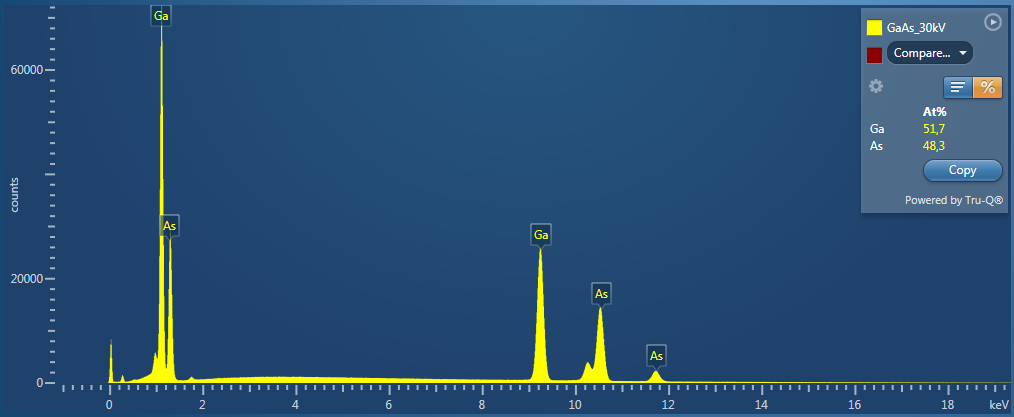
\includegraphics[width=0.95\textwidth]{figures/GaAs_30kV_SEM_lin.PNG}
    \\[2em]
    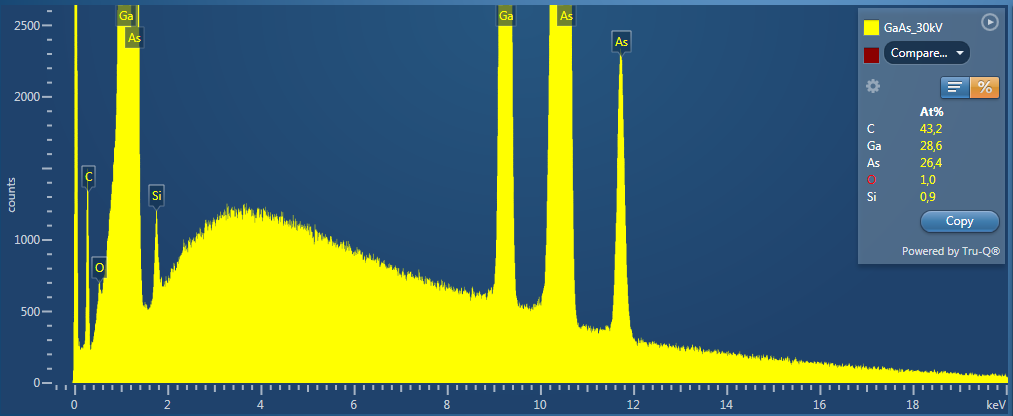
\includegraphics[width=0.95\textwidth]{figures/GaAs_30kV_SEM_lin_scaled.PNG}
    \\[2em]
    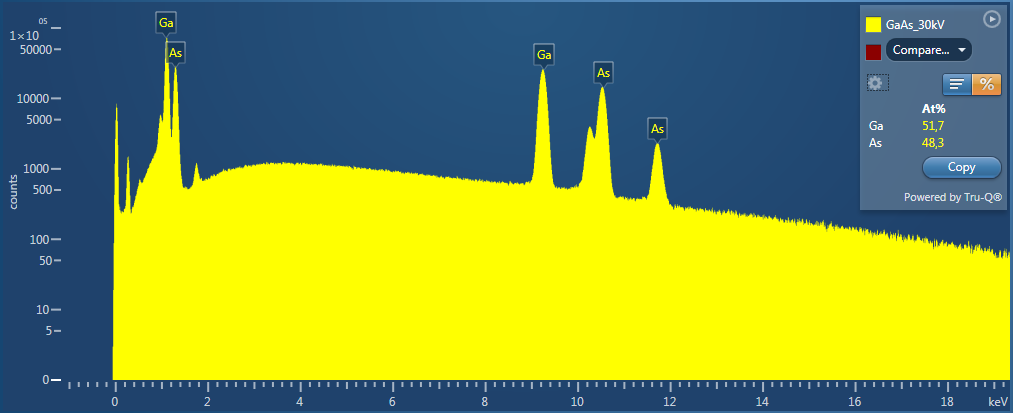
\includegraphics[width=0.95\textwidth]{figures/GaAs_30kV_SEM_log.PNG}
    \caption{
        The spectrum of the GaAs bulk at 30 kV, from AZtec.
        The figure shows the whole spectrum with Ga and As annotated, and a cropped version to show the smaller peaks where Si, O and C also are annotated.
        The bottom plot is the whole spectrum with a logarithmic scale on the y-axis.
    }
    \label{fig:GaAs30kV_AZ}
\end{figure}


% add figure figures/GaAs30kV_HS.png
\begin{figure}[p]
    \centering
    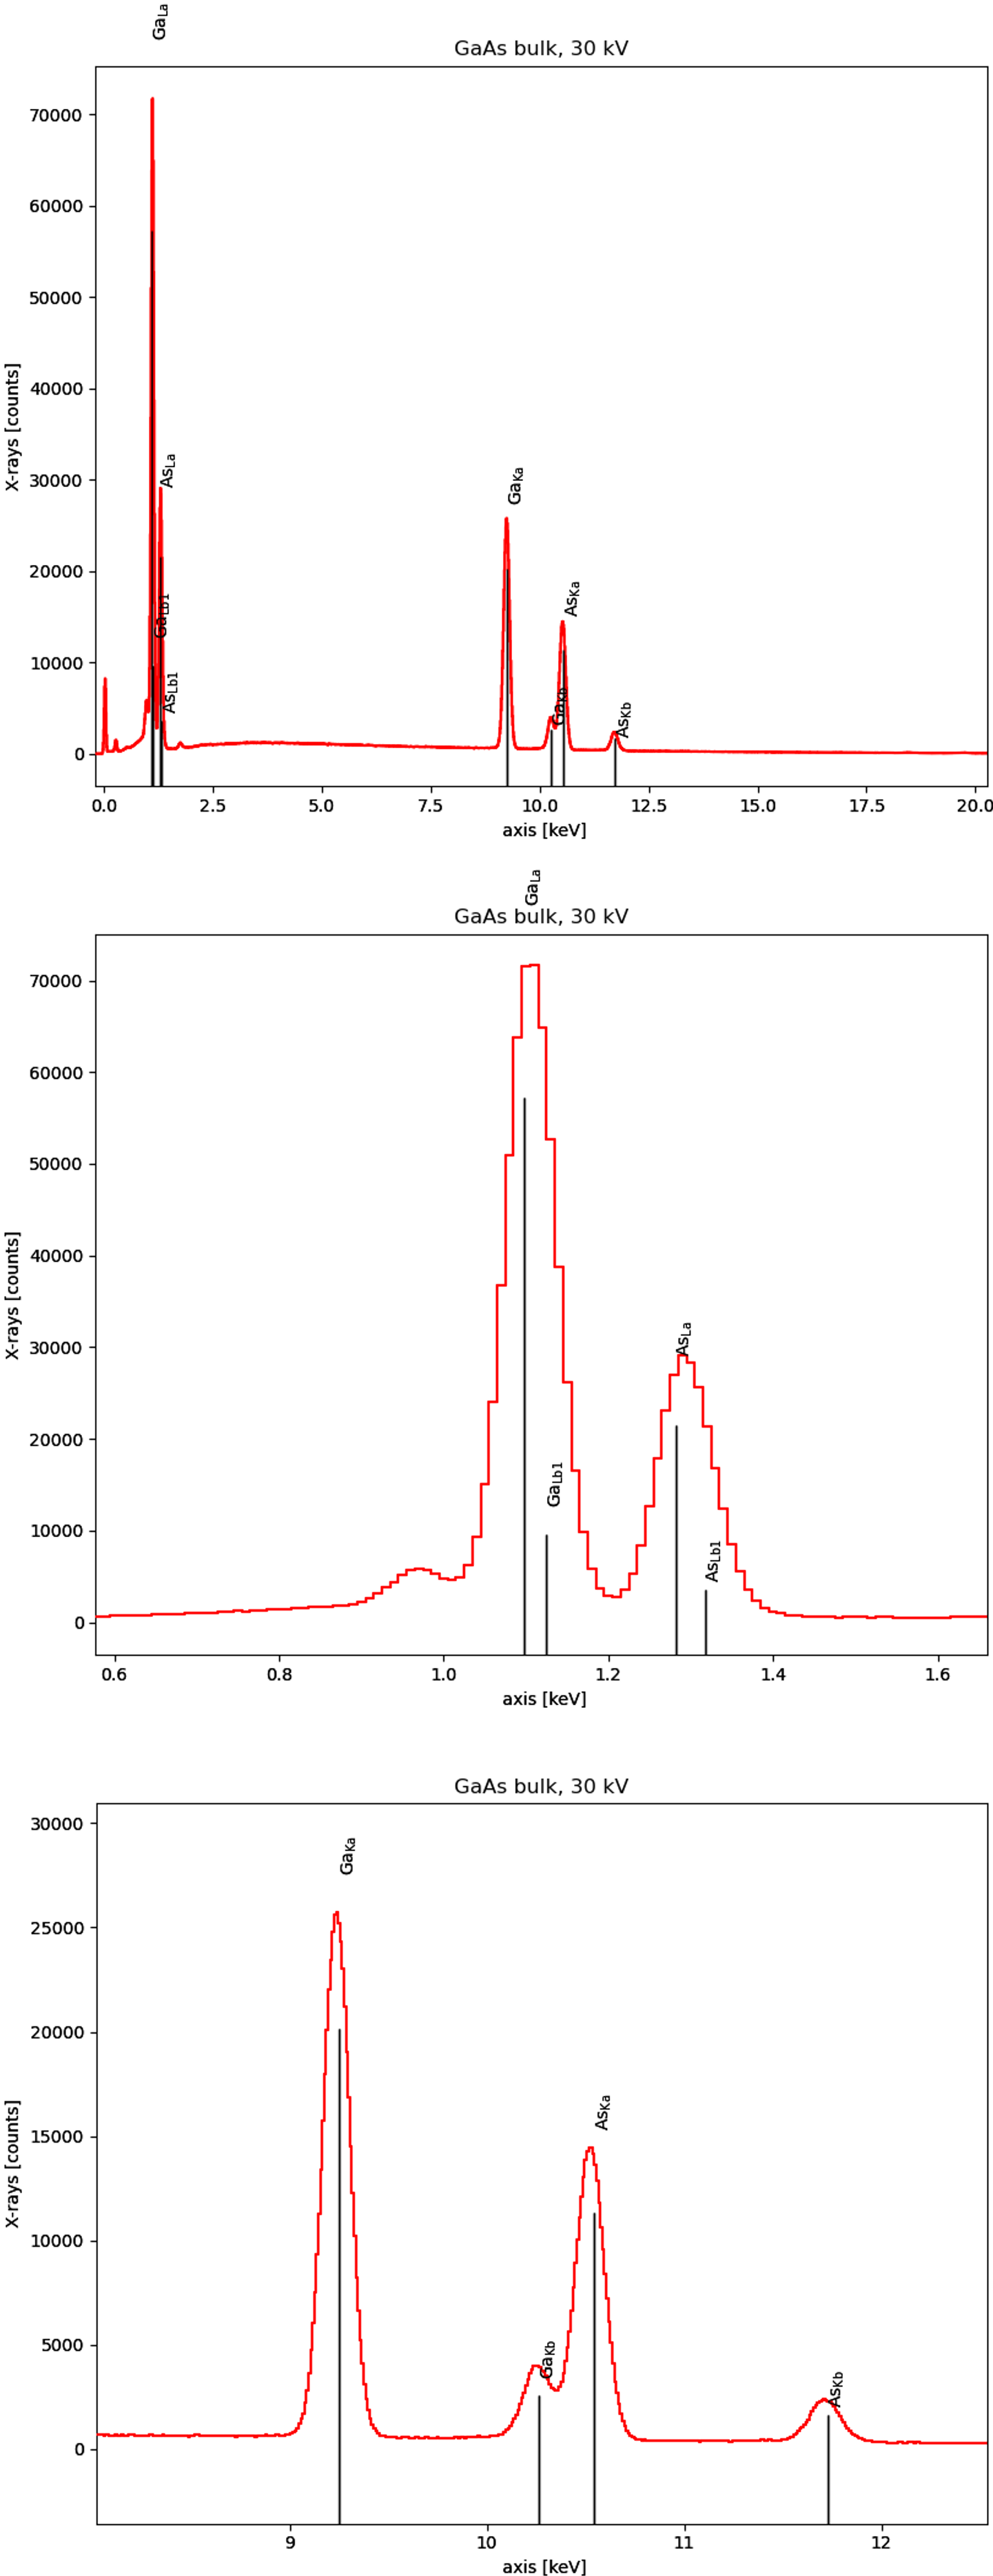
\includegraphics[width=0.95\textwidth]{figures/GaAs30kV_HS.png}
    \caption{
        The GaAs bulk spectrum taken at 30 kV, plotted with HyperSpy.
        The vertical lines are the theoretical peak centers.%, with weights as heights.
        (a) whole spectrum.
        (b) cropped to the L-peaks.
        (c) cropped to the K-peaks.
        (d) Ga K$\alpha$ peak.
        % This plot has the calibration from AZtec, and it is clear that the line position is deviating from the center of the peaks.
        % This plot was made with HyperSpy, which utilize Matplotlib.
    }
    \label{fig:GaAs30kV_HS}
\end{figure}






% qualitative results, calibration
\subsection{Calibration}
\label{sec:results:qualitative:calibration}

% what I did to calibrate the spectra
Different calibrations were explored.
The initial calibration is the one from AZtec, and is the one used in the spectra in \cref{fig:GaAs30kV_HS}.
The AZtec calibration has a left shift for the L-peaks and a right shift for the K-peaks.
The second type of calibration is the one given by the model fit in HyperSpy.
The third type is from the self-made model fit, using the distance between two high intensity and far apart peaks to calibrate the energy scale.
The third type use Ga L$\alpha$ and As K$\alpha$ peaks in the GaAs 30 kV spectrum, and use Mo L$\alpha$ and Mo K$\alpha$ peaks in the Mo 30 kV spectrum.

% the values
Values for the four calibrations are given in \cref{tab:results:calibrations}, i.e. the dispersion and the offset.
The deviations are a some eV, and the accuracy of the different calibrations give on specific peaks are given in \cref{tab:results:calibration-peak-accuracy}.
Here accuracy is the difference between the theoretical peak position and the peak center in the spectrum, given in eV.
The percentage deviation is also given.
At the bottom of the table the root-mean-square deviation (RMSD) is given.
For almost all the peaks, the deviation is greatest for the AZtec calibration.
One exception is the C K$\alpha$ peak, which deviates a lot less for the AZtec calibration. %discussion: Aztec might use the zero peak to calibrate, but that is just speculation.
The difference between the HyperSpy calibration and the self-made calibration on the GaAs is small.
In the qualitative section, the effect of the different calibrations on the spectra are explored.
% Discuss: even though Mo is further apart, this calibration is worse than GaAs

% dispersion and offset table
% Calibration values
% chapter Results
\begin{table}[ht]
    \centering
    \caption{
        Different calibration values.
        The AZtec calibration is reffered to as the uncalibrated value.
        The dispersion is calculated with \cref{eq:theory:calibration:dispersion}.
        The offset is calculated with \cref{eq:theory:calibration:offset}.
        The own calibration was done on Ga L$_\alpha$ and As K$_\alpha$ from the 30 kV measurement on the GaAs wafer.
        The HyperSpy cailbration was done by making a model and fitting it to the data on the 30 kV GaAs spectrum.
    }
    \label{tab:results:calibrations}
    % \begin{tabular}{m{4cm} m{2cm} m{2cm}}
    \begin{tabular}{ccc}
        Calibration method & Dispersion,   & Zero offset \\
                           & [keV/channel] & [channels]  \\
        \hline
        AZtec              & 0.01          & 20          \\
        HyperSpy           & 0.010028      & 21.0787     \\
        Own calibration    & 0.010030      & 21.127
    \end{tabular}
\end{table}


% calibration peak accuracy table
% table with peak accuracy

\begin{table}[p]
    \centering
    \caption{
        % TODO: give the peak accuracy in ev, not percent. Or eV and percent?
        Peak accuracy of the different calibration methods on 30 kV spectra: NW, Mo, Si, Al, Cu. % TODO: reformulate
        The other acceleration voltages gave similar results.
        The accuracy here is the deviation from the theoretical peak to the measured peak.
        The percentage deviation is also given.
        The measured peak is the fitted center of the peak.
        % discussion: The Mo L$\alpha$ deviates much because the peak is not well fitted.
        % The C K$\alpha$ is fitted well, but deviates much more than all the other peaks.
        The self-made calibration was done on two spectra: GaAs and Mo. % discussion: Mo is more far apart than GaAs.
        % One was done on Ga L$\alpha$ and As K$\alpha$ from the 30 kV measurement on the GaAs wafer.
        % The other was done on the more far apart peaks Mo L$\alpha$ and Mo K$\alpha$ from the 30 kV measurement on the Mo wafer.
        The HyperSpy calibration was done on the GaAs spectrum.
        At the bottom the RMS of the deviation in the column is given.
    }
    \label{tab:results:calibration-peak-accuracy}
    \begin{tabular}{cccccc}
        Peak         & Theoretical & AZtec                 & HyperSpy              & Ga L$\alpha$ \& As K$\alpha$ & Mo L$\alpha$ \& Mo K$\alpha$ \\
                     & [keV]       & [eV]                  & [eV]                  & [eV]                         & [eV]                         \\
        \hline
        As L$\alpha$ & 1.2819      & 12.8,\,\,\,    1.0\%  & 5.6,\,\,\,    0.4\%   & 5.4,\,\,\,    0.4\%          & 7.2,\,\,\,    0.6\%          \\
        As K$\alpha$ & 10.5436     & -21.3,\,\,\,   -0.2\% & -2.7,\,\,\,   -0.0\%  & -1.1,\,\,\,   -0.0\%         & 9.8,\,\,\,    0.1\%          \\
        Ga L$\alpha$ & 1.098       & 11.5,\,\,\,    1.0\%  & 3.8,\,\,\,    0.3\%   & 3.5,\,\,\,    0.3\%          & 5.1,\,\,\,    0.5\%          \\
        Ga K$\alpha$ & 9.2517      & -14.2,\,\,\,   -0.2\% & 0.9,\,\,\,    0.0\%   & 2.2,\,\,\,    0.0\%          & 11.9,\,\,\,    0.1\%         \\
        Cu L$\alpha$ & 0.9295      & 16.4,\,\,\,    1.8\%  & 8.3,\,\,\,    0.9\%   & 8.0,\,\,\,    0.9\%          & 9.4,\,\,\,    1.0\%          \\
        Cu K$\alpha$ & 8.0478      & -9.2,\,\,\,   -0.1\%  & 2.5,\,\,\,    0.0\%   & 3.7,\,\,\,    0.0\%          & 12.1,\,\,\,    0.2\%         \\
        Mo K$\alpha$ & 17.4793     & -56.8,\,\,\,   -0.3\% & -18.8,\,\,\,   -0.1\% & -15.8,\,\,\,   -0.1\%        & 1.9,\,\,\,    0.0\%          \\
        Mo L$\alpha$ & 2.2932      & 24.0,\,\,\,    1.0\%  & 19.7,\,\,\,    0.9\%  & 19.7,\,\,\,    0.9\%         & 22.5,\,\,\,    1.0\%         \\
        Si K$\alpha$ & 1.7397      & 2.9,\,\,\,    0.2\%   & -3.0,\,\,\,   -0.2\%  & -3.2,\,\,\,   -0.2\%         & -1.0,\,\,\,   -0.1\%         \\
        Al K$\alpha$ & 1.4865      & 3.0,\,\,\,    0.2\%   & -3.7,\,\,\,   -0.2\%  & -3.9,\,\,\,   -0.3\%         & -1.9,\,\,\,   -0.1\%         \\
        Cu K$\alpha$ & 8.0478      & -9.3,\,\,\,   -0.1\%  & 2.4,\,\,\,    0.0\%   & 3.5,\,\,\,    0.0\%          & 11.9,\,\,\,    0.1\%         \\
        C K$\alpha$  & 0.2774      & -8.2,\,\,\,   -3.0\%  & -18.3,\,\,\,   -6.6\% & -18.7,\,\,\,   -6.7\%        & -17.9,\,\,\,   -6.5\%        \\
        \hline
        RMS  [eV]    &             & 14.75                 & 4.62                  & 4.55                         & 9.57
    \end{tabular}
\end{table}


% Peak finding and fitting
For the third type of calibration, the peaks were located and fitted to Gaussians, and the background was fitted as a polynomial.
The fit of the 30 kV GaAs spectrum is shown in \cref{fig:results:fit_GaAs30kV}.
The fit was done with a background polynomial of order 6 and 12, and both the fit and the background is plotted.
Some peaks had too low prominence to be detected by \verb|scipy.signal.find_peaks|, like the Si K$\alpha$ peak.
The accuracy of the fit was quantified as the root-mean-square error (RMSE) between the fitted curve and the data, and the RMSE is given in the subplots.

% discuss: the fit is best at 12th order. The fit is quite good, but two things to improve are the peak finder and the shape of the background.

% make figure with 4 subfigures.
% fit_GaAs30kV_whole.png
% fit_GaAs30kV_K.png
% fit_GaAs30kV_L.png
% fit_GaAs30kV_bg.png

\begin{figure}[p]
    \centering
    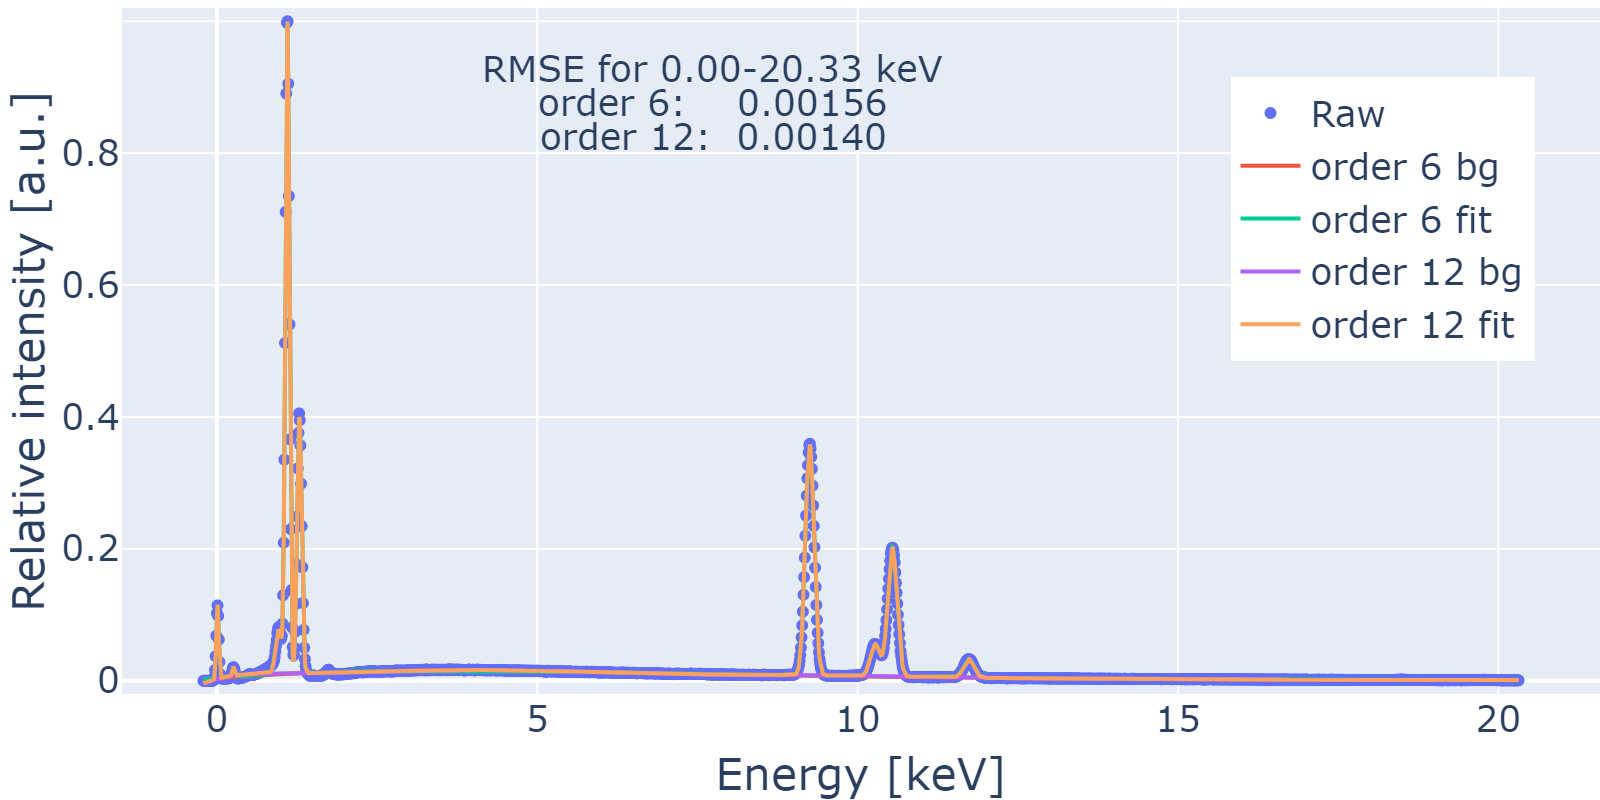
\includegraphics[width=0.48\textwidth]{figures/fit/fit_GaAs30kV_whole.png}
    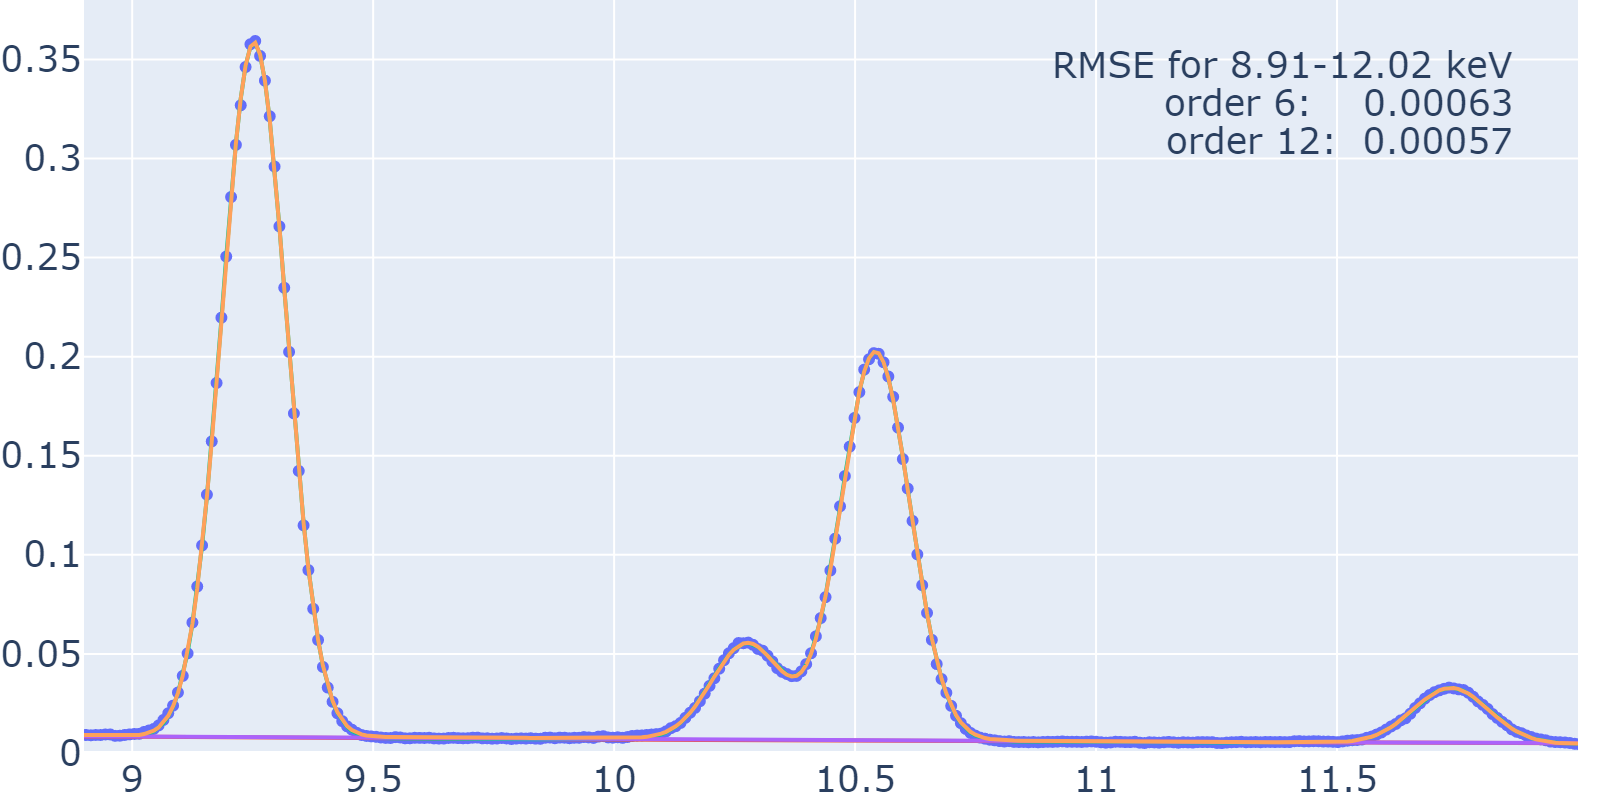
\includegraphics[width=0.48\textwidth]{figures/fit/fit_GaAs30kV_K.png}
    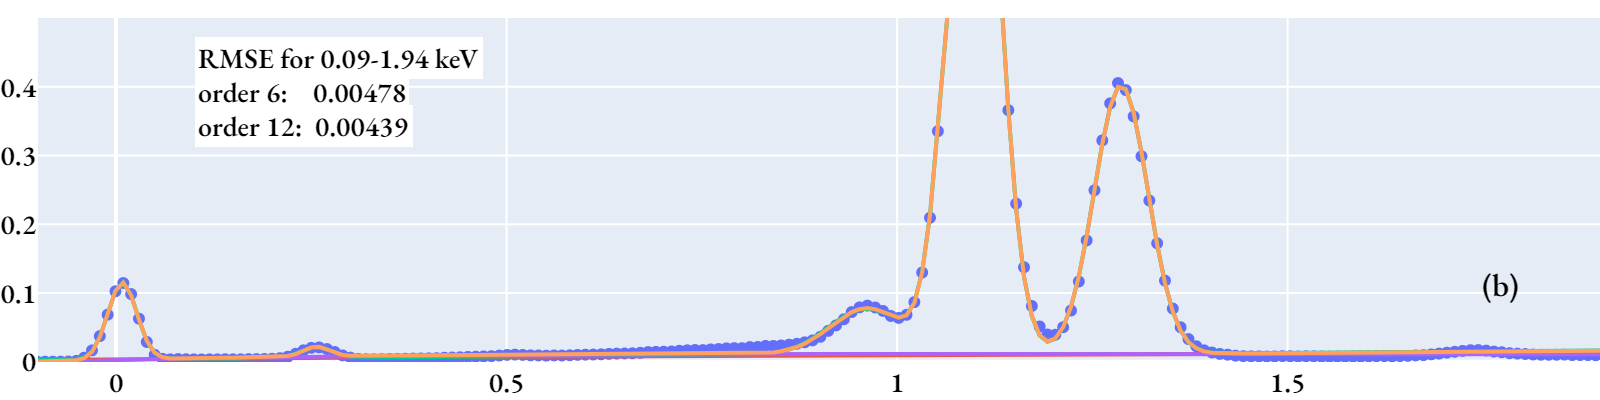
\includegraphics[width=0.48\textwidth]{figures/fit/fit_GaAs30kV_L.png}
    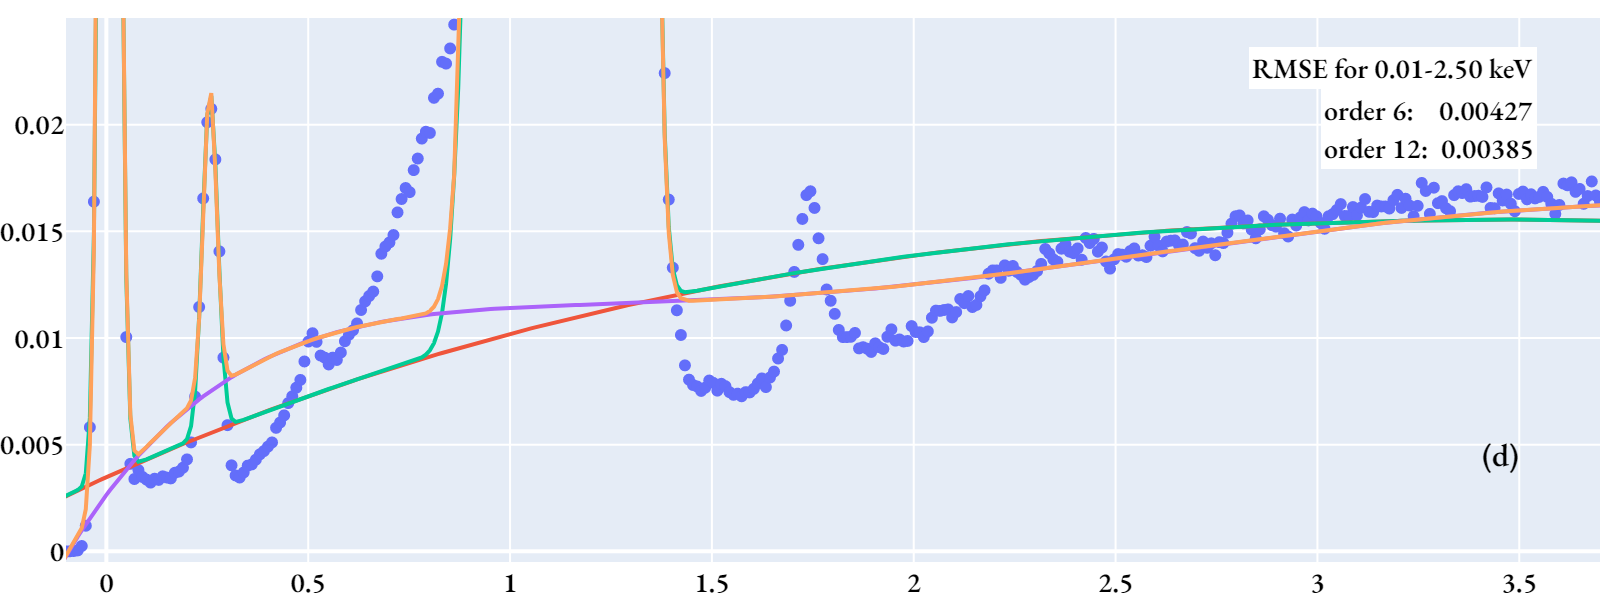
\includegraphics[width=0.48\textwidth]{figures/fit/fit_GaAs30kV_bg.png}
    \caption{
        The fit of the 30 kV GaAs spectrum.
        The plots show the raw data (blue markers), the fit (green and orange) and he background (red and purple).
        The two different fits and backgrounds are with background polynomial of order 6 and 12, respectively.
        The RMSE for the area of each plot is given on the figures.
    }
    \label{fig:results:fit_GaAs30kV}
\end{figure}


% newpage before next section
\newpage

\subsection{Spectra from the studied materials}
\label{sec:results:qualitative:each_sample_area}

% The goal of this section/the qualitative analysis is ... 
\cref{fig:results:Spectra_Al} to \cref{fig:results:Spectra_NW} shows the spectra for the six different areas of the sample plotted with Plotly.
The plots are available as an interactive HTML plots on the GitHub repository
% \brynjar{Upload the HTML files to the GitHub repository.}.
The calibration used in these spectra is one with the lowest RMSD, which is the one from the self-made model fit on GaAs.
The y-axis is normalized to the highest peak value in each spectrum, i.e. the highest peak is always 1. % discuss: why normalize.
The spectra are cropped to show the region of interest for the different materials.
Peaks which are taller than the y-axis are marked with a gray dashed line.
The annotated energy on the plots is the theoretical energy of the peak, and not the fitted peak center.
Some black annotation lines are visually off center on the peaks, which is due to the peak deviation previously shown in \cref{tab:results:calibration-peak-accuracy}.
The terms peak and signal is used to differentiate between well-defined peaks and signals with low signal-to-noise ratio.
The differentiation between peak and signal is not quantified with a threshold in this work. % discuss: could be done, but needs to be tested. Might be able to determine certain peaks from stray peaks, idk.
The annotations with an asterisk (*) are the peaks which have not theoretical value, e.g. a sum peak.
First the spectra from the pure samples are presented, then the GaAs bulk wafer, and finally the GaAs NW.
The order are: Al, Si, Cu, Mo, GaAs bulk, GaAs NW.


% Al alloy is normally with Mg and Si, while Mn is not that common. Can discuss if Si is stray or in the alloy.


% figure Spectra_Al.png
\begin{figure}[b!]
    \centering
    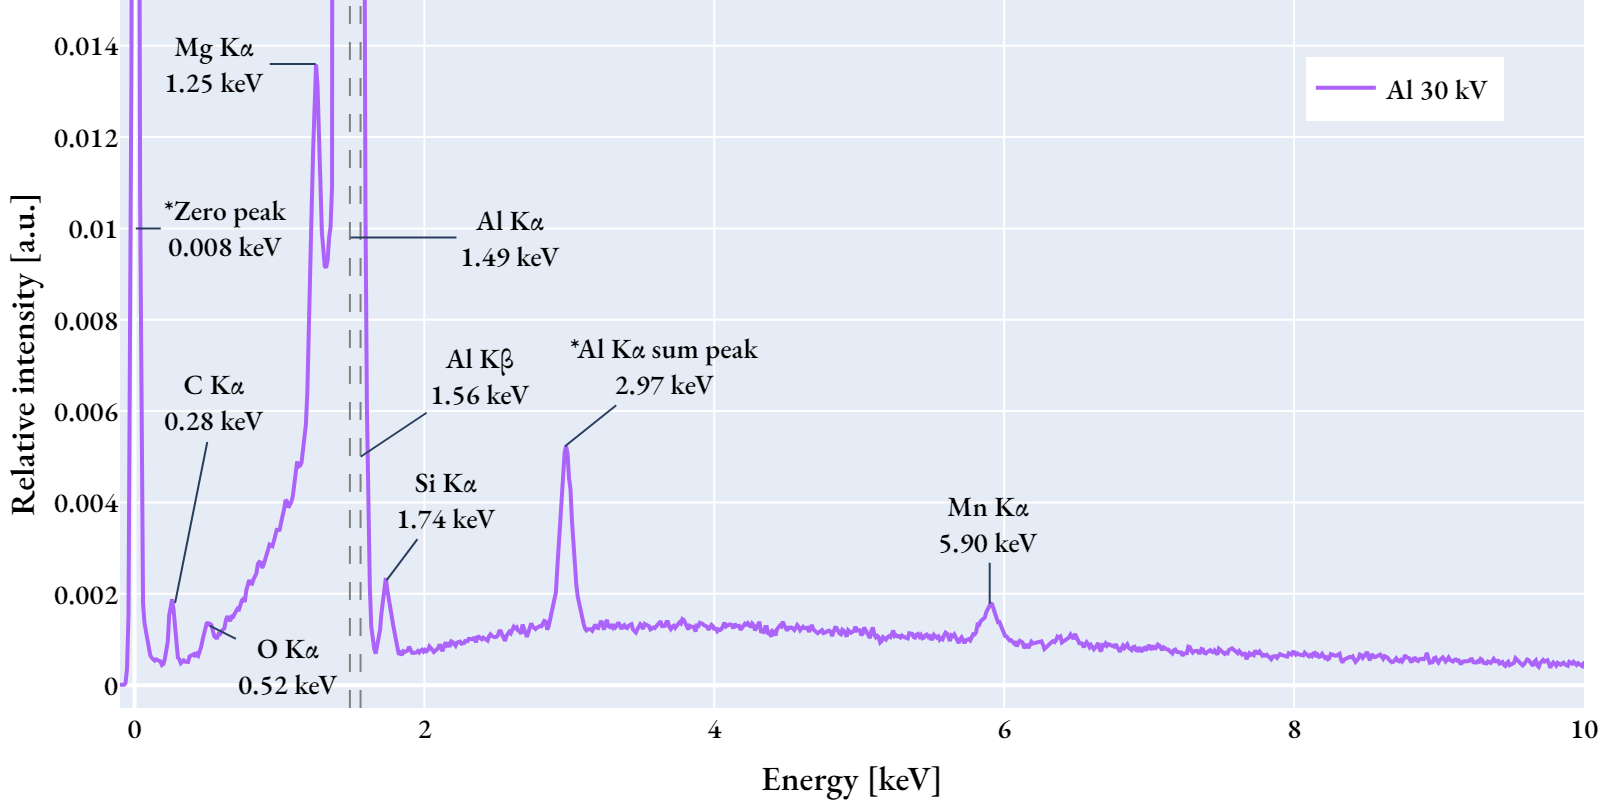
\includegraphics[width=0.90\textwidth]{figures/each_spectra/Al_everything.png}
    \caption{
        % What the sample is. The legen colors, What is annotated. Special features present are peaks, sum peaks and eventually unknown peaks. Spectra taken ... 
        The 30 kV spectrum from the Al FIB stub.
        The peaks are annotated with the theoretical energy.
        The sum peak and zero peak are annotated with an asterisk, as they do not have a theoretical value.
        The dashed lines mark Al K$\alpha$ and K$\beta$, which together form one peak with relative intensity 1.
        % The tallest peak is at 1.49 keV, and it is the Al K$\alpha$ peak with some signal at the K$\beta$ peak at 1.56 keV.
        % The relative weight for Al K$\beta$ to K$\alpha$ is 0.013 (from HyperSpy).
        % Fe K$\alpha$ at 6.40 keV has a question mark, because the FIB stub was initially expected to be Fe.
        % The signal from Fe K$\alpha$ is barely a signal different from the background.
    }
    \label{fig:results:Spectra_Al}
\end{figure}
% The Al spectra
The Al spectrum from the FIB stub is shown in \cref{fig:results:Spectra_Al}.
As all the other spectra, this spectrum have a zero peak, a C K$\alpha$ peak at 0.260 keV and a O K$\alpha$ peak at 0.51 keV.
Most of the other spectra also have a Si K$\alpha$ peak at 1.74 keV.
The tallest peak with a relative intensity of 1 is the combined peak of Al K$\alpha$ and K$\beta$ at 1.49 keV.
The contribution of Al K$\beta$ to Al K$\alpha$ is 0.013, which is small, but still changes the peak shape.
% The FIB stub was initially expected to be Fe, but the spectrum lacks a Fe K$\alpha$ peak at 6.40 keV.
There are some signal at 6.40 keV, which is where Fe K$\alpha$ would be, but here the signal-to-noise level is low.
The signal at 6.40 keV is around 20\% higher than the background, where the background have counts from 150-180 and the signal has 210-220 counts.
The peaks at 1.25 keV and 5.9 keV indicate that there was Mg and Mn in the sample, either as impurities or as part of the alloy.
% discussion: Al-Mg-Mn alloy, but unable to quantify with my bad signal, or?
% discussion: Mn not common, says Ton, but Mg and Si is common in Al alloy.
The last peak in the spectrum is the Al K$\alpha$ sum peak at 2.97 keV. % discussion: what other peaks could this be.
The background is increase rapidly and almost linearly from C K$\alpha$ to Al K$\alpha$, and drops to 10\% after the Al K$\alpha$ peak.
The figure also show that the Al K$\alpha$ absorbs part of the background to the right of the peak.



% The Si spectra
The Si spectra from the pure Si wafer sample area is shown in \cref{fig:results:Spectra_Si}.
As in the other spectra, this spectrum have a zero peak, a C K$\alpha$ peak at 0.260 keV and a O K$\alpha$ peak at 0.51 keV.
In addition, there is an unidentified peak at 0.080 keV.
The tallest peak with a relative intensity of 1 is the Si K$\alpha$ peak at 1.73 keV, which have a contribution from the K$\beta$ peak at 1.84 keV.
The relative weight for Si K$\beta$ to K$\alpha$ is 0.028.
As in the Ai spectrum, the Si spectra have a sum peak from the tallest peak.
The sum peak is at 3.48 keV, which is the sum peak of the Si K$\alpha$.
In all four spectra the background drops significantly after the Si K$\alpha$ peak.
The relative drop down is biggest in the 30 kV spectrum.
The plot show that the background level is dependent on the acceleration voltage, at least when the spectrum is normalized to the tallest peak.
% Discussion: normalization/sum peaks/DT: can mention the "odd" ratios of the Si sum peak, where 10 kV is tallest, then 30, then 5 and 15 at the same level. This is due to normalization and the fact that the DT was not equal. Use table in methods to show the DT.


% figure Spectra_Si.png
\begin{figure}[h!]
    \centering
    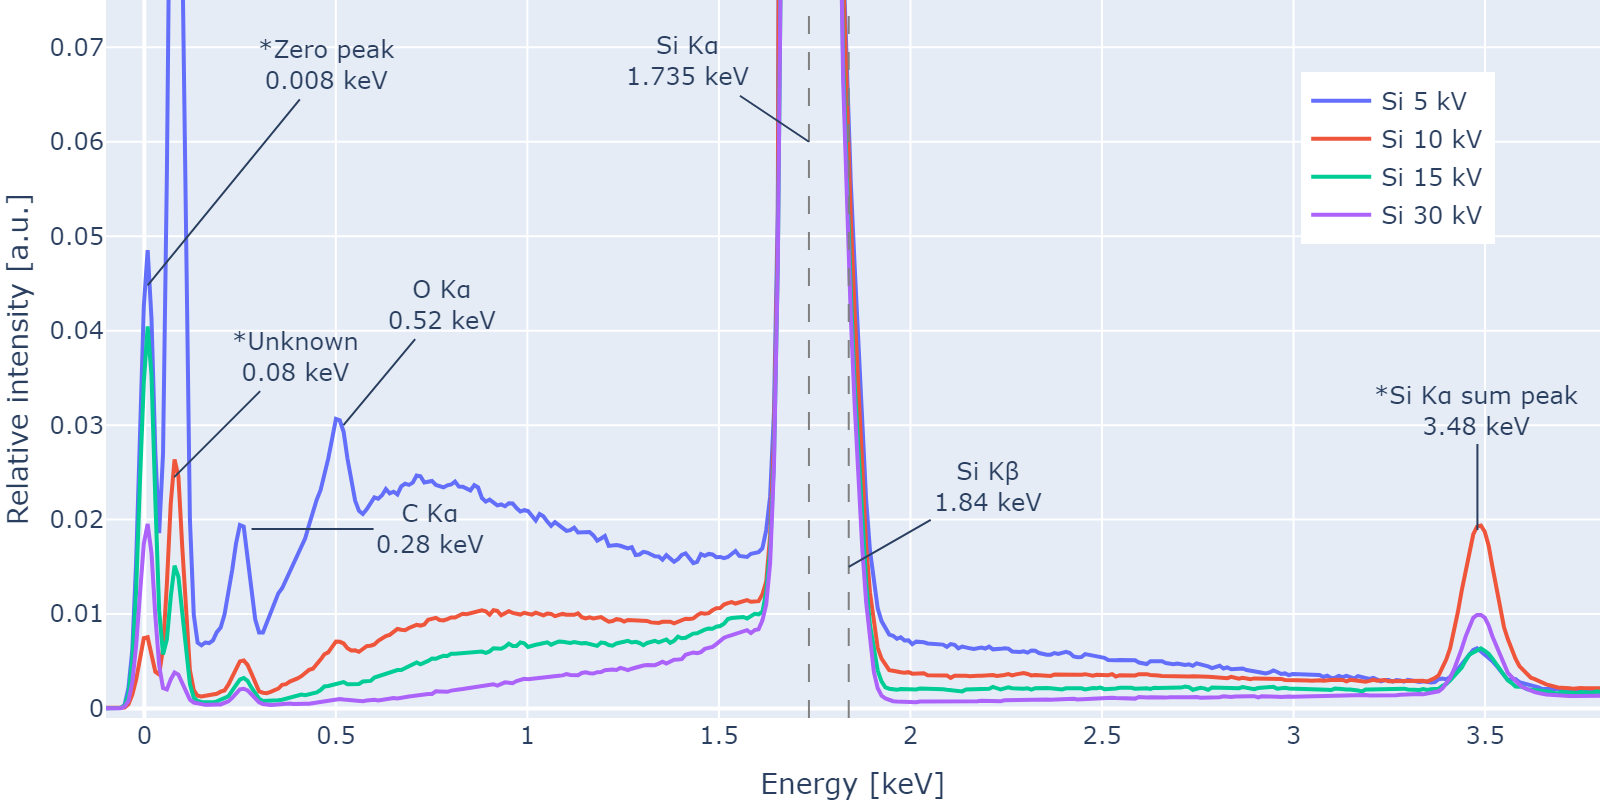
\includegraphics[width=0.90\textwidth]{figures/each_spectra/Si_everything.png}
    \caption{
        The spectra of the Si wafer, taken at 5 (blue), 10 (red), 15 (green), and 30 (purple) kV.
        The peaks are annotated with the theoretical energy.
        The sum, unknown and zero peak are annotated with an asterisk, as they do not have a theoretical value.
        The dashed lines mark Si K$\alpha$ and K$\beta$, which together form one peak with relative intensity 1.
    }
    \label{fig:results:Spectra_Si}
\end{figure}



% The Cu spectra
The Cu spectra from the Cu-tape is shown in \cref{fig:results:Spectra_Cu}.
These spectra have a zero peak, a C K$\alpha$, a O K$\alpha$ peak and a small Si K$\alpha$ peak.
The tallest peak with a relative intensity of 1 is the C K$\alpha$ peak at 0.26 keV.
The Cu K$\alpha$ and Cu K$\beta$ peaks are only visible at the 30 kV spectrum.
The height of the Cu K$\alpha$ peak is 0.017, which means that the C K$\alpha$ peak is more than 55 times taller.
None of the spectra have a Cu L$\alpha$ peak, which should have been at 0.93 keV.
The 30 kV spectrum have a signal at 2.29 keV, which could be from Mo L$\alpha$, but no Mo K$\alpha$ signal is visible.
% discussion: The other spectra show that the L peaks are taller. No singal except noise at all at 17.48 keV. But the Mo La peak is low, so it makes sense.
In these spectra the background is highest at the 30 kV spectrum, which is the opposite as for the Si spectra.
The peak heights look dependent on the acceleration voltage, but the plot hides the fact that the DT is not equal for all spectra.
% Discussion: what makes the peaks high and low? This is to be able to get good data, but at the same time not getting biased data by forcing some special stuff.


% figure Spectra_Cu.png
\begin{figure}[h]
    \centering
    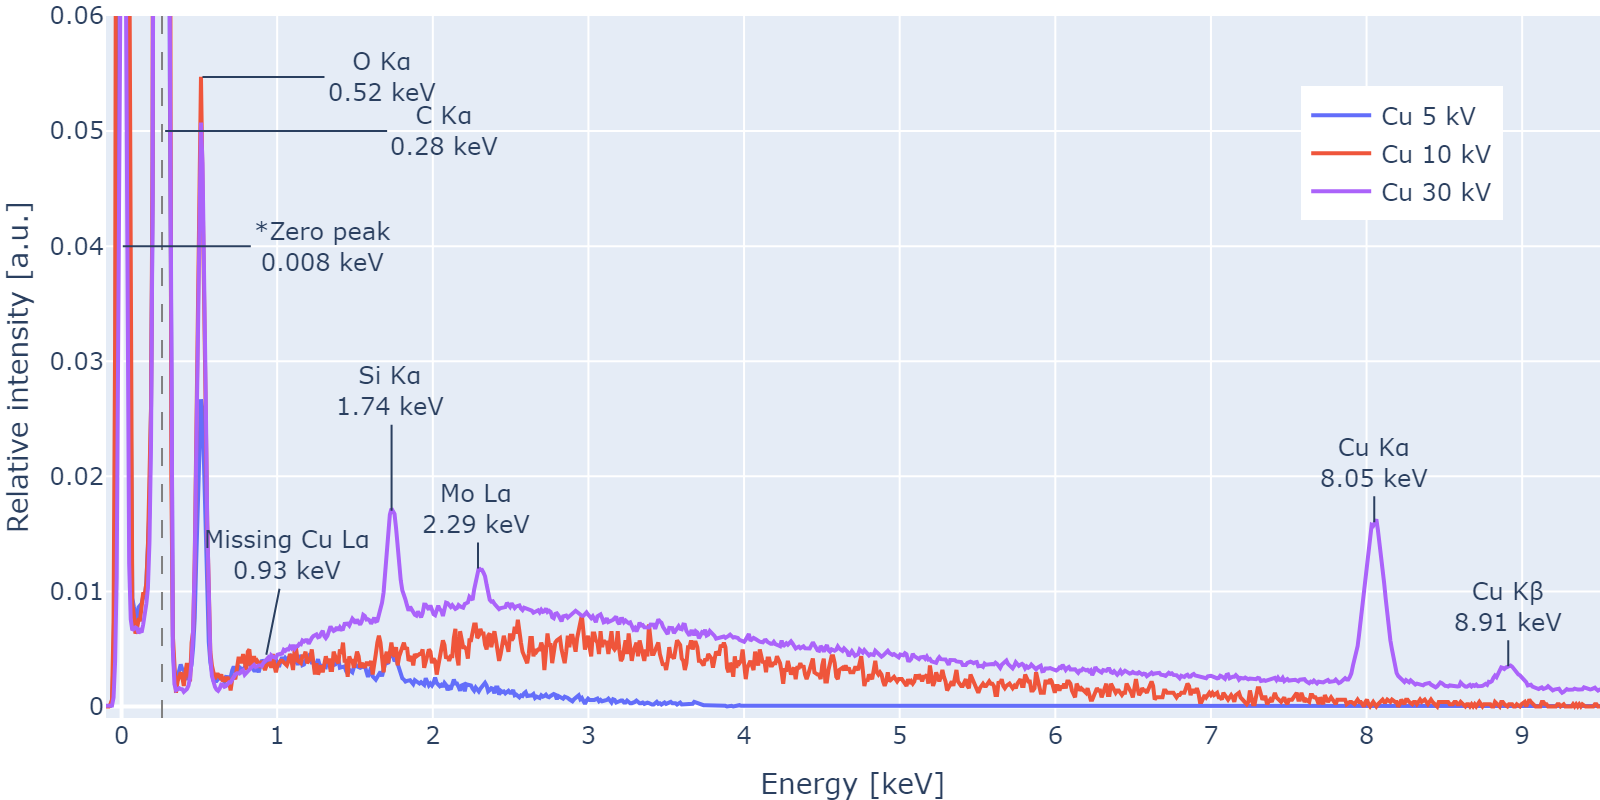
\includegraphics[width=0.90\textwidth]{figures/each_spectra/Cu_everything.png}
    \caption{
        The spectra of the Cu-tape, taken at 5 (blue), 10 (red), and 30 (purple) kV.
        The peaks are annotated with the theoretical energy.
        The zero peak is annotated with an asterisk, as it does not have a theoretical value.
        The dashed line mark the C K$\alpha$ peak.
        The expected, but missing, Cu L$\alpha$ peak is marked.
    }
    \label{fig:results:Spectra_Cu}
\end{figure}

% figure Spectra_Mo.png
\begin{figure}[b!]
    \centering
    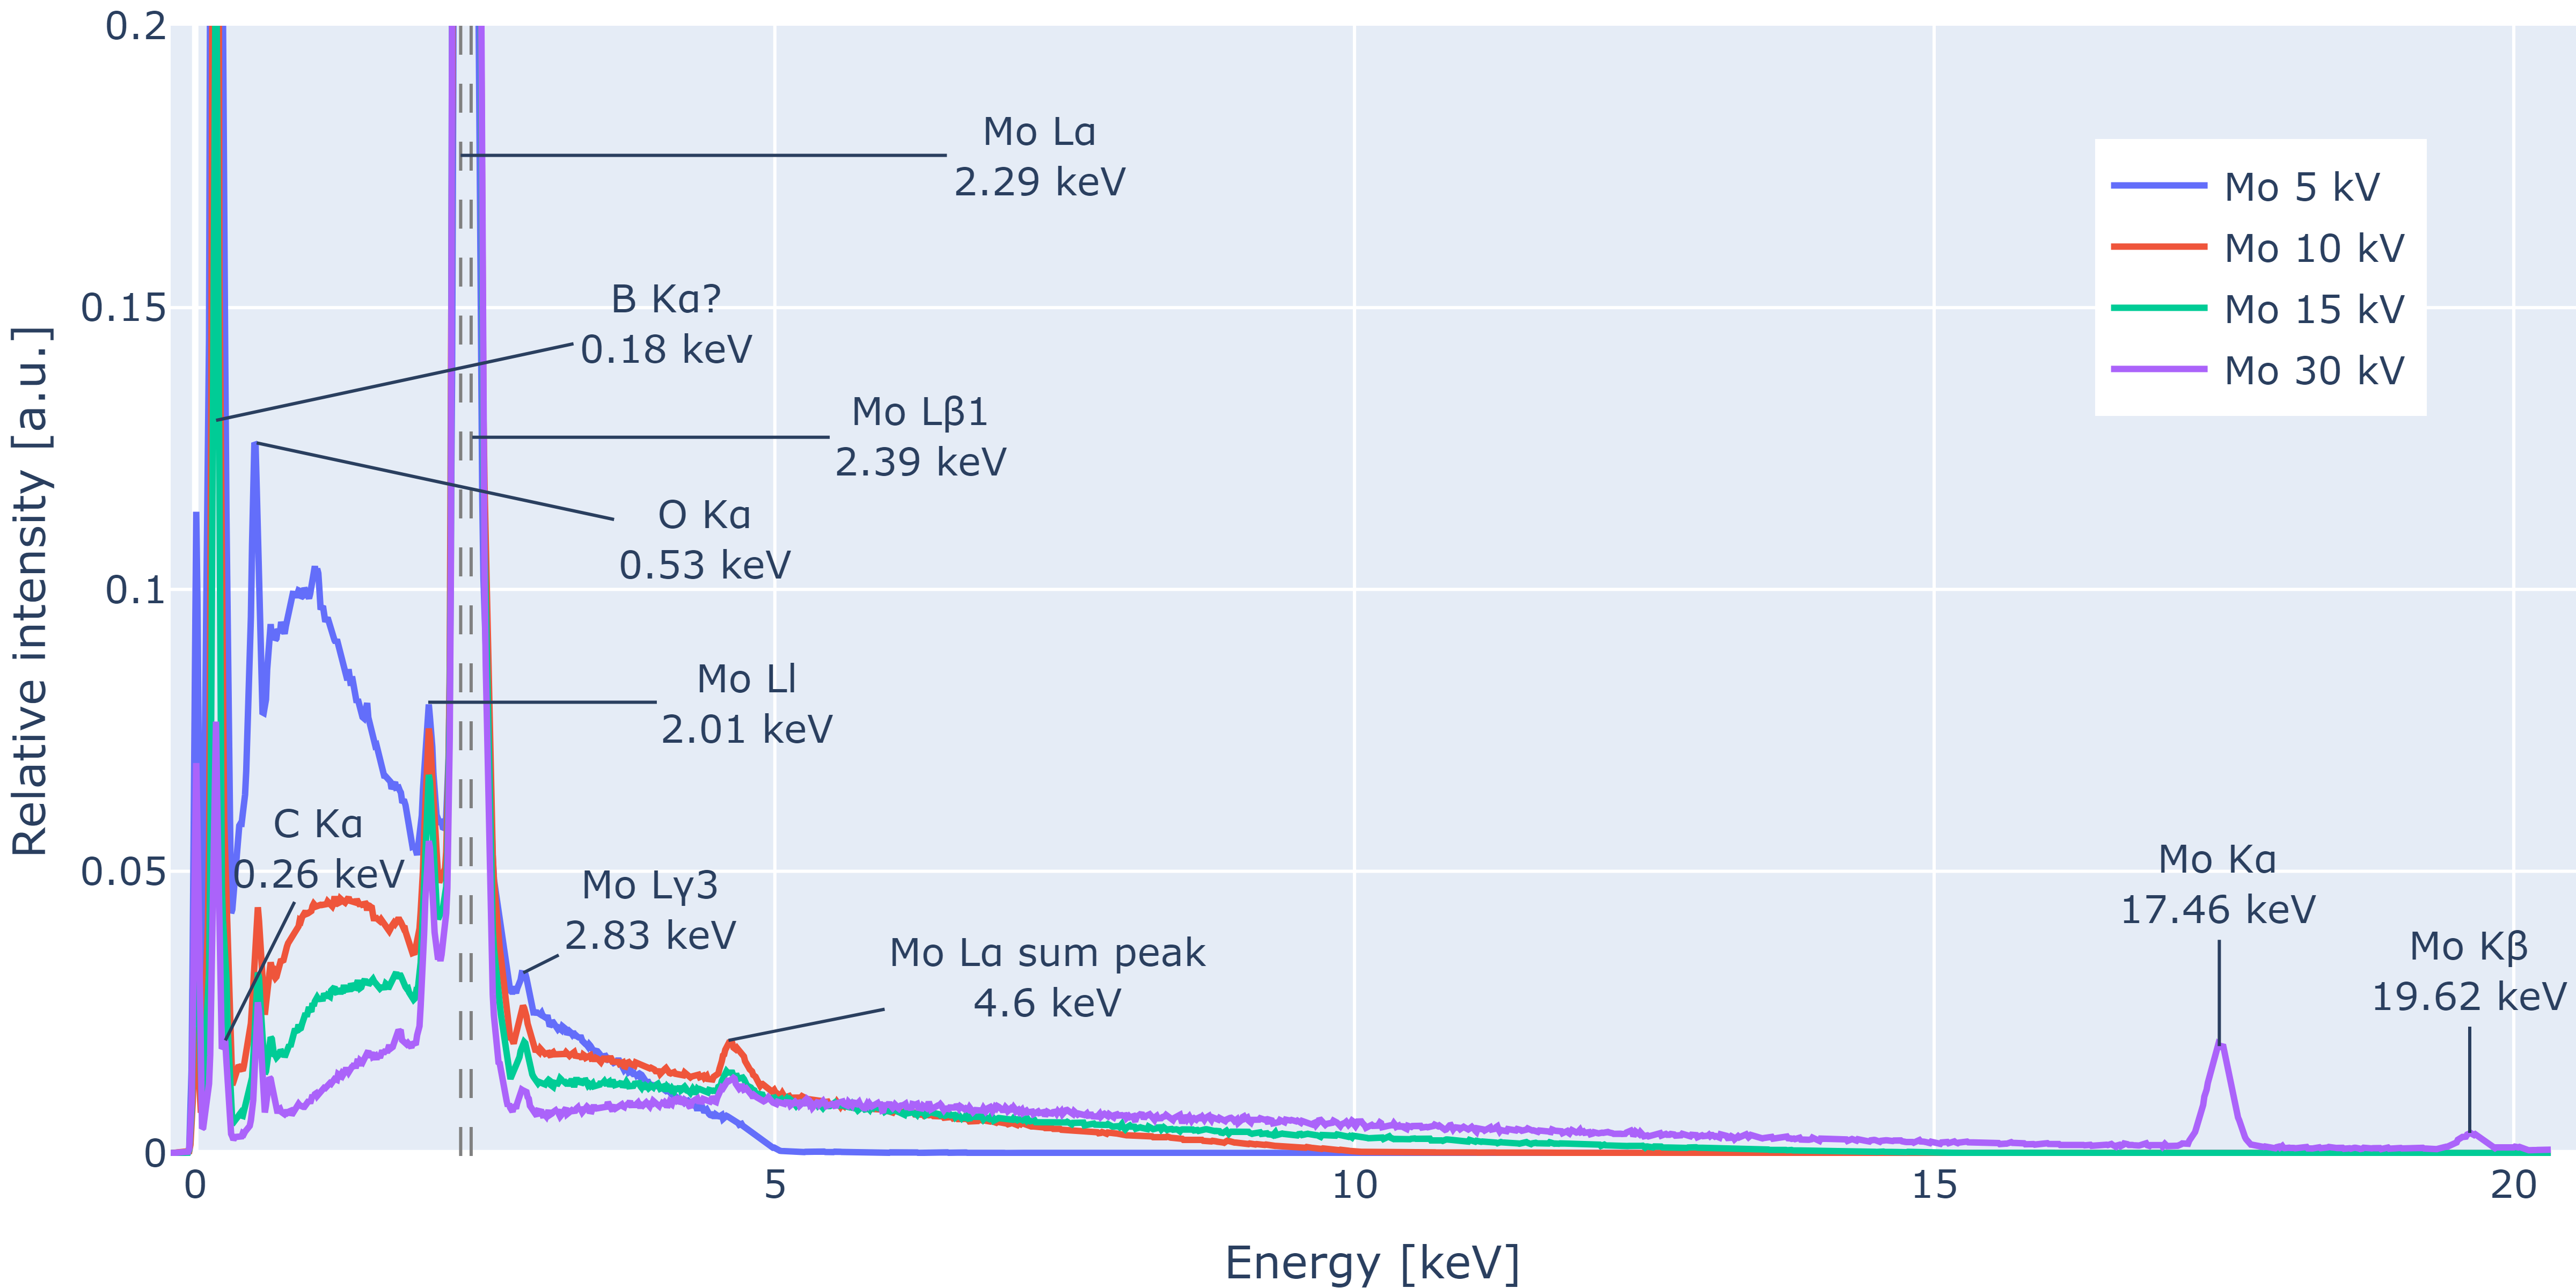
\includegraphics[width=0.90\textwidth]{figures/each_spectra/Mo_everything.png}
    \caption{
        The spectra of the Mo disk, taken at 5 (blue), 10 (red), 15 (green), and 30 (purple) kV.
        The peaks are annotated with the theoretical energy.
        The sum, unknown and zero are annotated with an asterisk, as they do not have a theoretical value.
        The dashed lines mark Mo L$\alpha$ and Mo L$\beta$1. %, which are barely distinguishable and have a relative intensity in the 30 kV spectrum of 1 and 0.45, respectively.
        The background of the 5 kV spectrum is higher than the other spectra, which is due to the normalization to the tallest peak. %, because the tallest peak in the 5 kV spectrum is not Mo L$\alpha$, but the peak at 0.18 keV.
    }
    \label{fig:results:Spectra_Mo}
\end{figure}



% The Mo spectra
The Mo spectra from the Mo disk are shown in \cref{fig:results:Spectra_Mo}.
The four spectra have a zero peak, a C K$\alpha$, a O K$\alpha$ peak.
The Si K$\alpha$ give a very small signal, and is visible as the tiny peak before Mo Ll.
The background of the 5 kV spectrum is very high, but that is due do its lower signal on the Mo L$\alpha$, making the 0.18 keV peak the tallest and thus scaling up the background.
In other words, the 5 kV spectrum is scaled to another peak, because the Mo L$\alpha$ peak is low. % discuss: overvoltage makes Mo La lower. Max signal is at more than U*2.
The tallest peak in the 5 kV spectrum is the 0.18 keV peak, which is also visible in the other three spectra.
The energy of 0.18 keV only match with the B K$\alpha$ line at 0.1833 keV. % discuss, it is really this peak? The accuracy is low at low E, use the talbe which show that C Ka miss a lot.
The tallest peak in the 10, 15 and 30 kV spectra is the Mo L$\alpha$ peak at 2.29 keV, which is contributed by the Mo L$\beta$1 peak at 2.39 keV.
This one peak consists of two overlapping Gaussian, which are barely distinguishable.
The HyperSpy database have the energy and weight of two other Mo peaks visible in the spectrum, which are the Mo Ll and Mo L$\gamma$3 peaks at 2.01 keV and 2.83 keV.
%
% TODO: write about the Mo Ll and Mo L$\gamma$3 peaks in the teory section.
%
The X-ray Booklet does not include these lines, but include some other lines which are not visible in these spectra.
This difference between the listed lines in the X-ray Booklet and the lines in the HyperSpy database can be confusing and is part of the discussion in \cref{chap:discussion}. % discuss: the difference might be that HS is more empirical while the X-ray Booklet is more theoretical.
% also give the cref a more direct reference
Only the 30 kV spectra have a signal at the Mo K$\alpha$ and Mo K$\beta$ peaks at 17.46 and 19.62 keV. % discuss: as expected
The peak at 4.6 keV is the sum peak of Mo L$\alpha$ and Mo L$\beta$1.
As in the other spectra, the background drops significantly after the tallest peak.


% figure Spectra_GaAs.png
\begin{figure}[b!] % p is to get their own page for floats
    \centering
    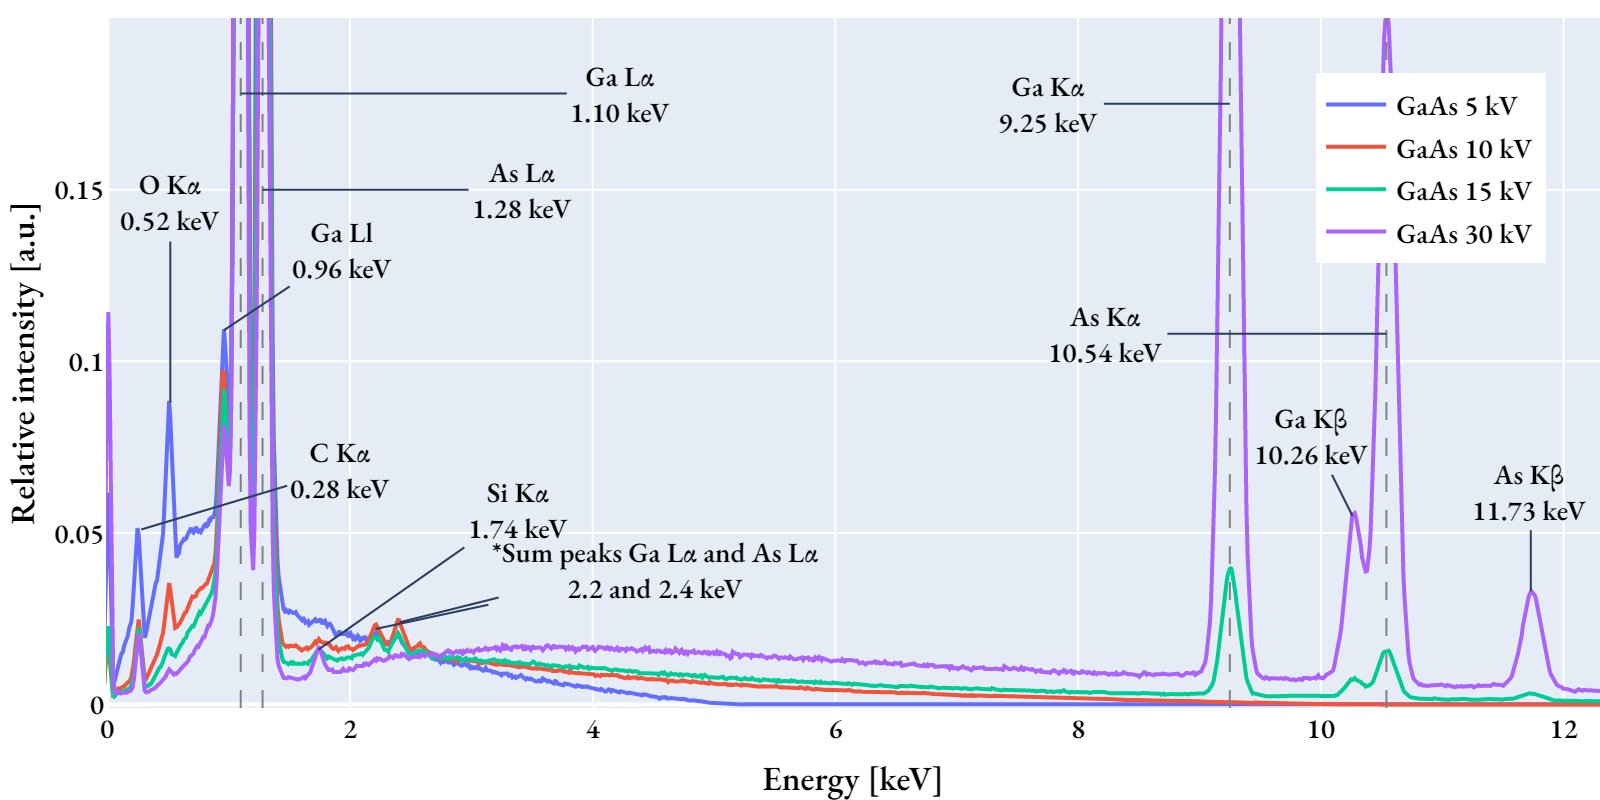
\includegraphics[width=0.90\textwidth]{figures/each_spectra/GaAs_everything.png}
    \caption{
        The spectra of the GaAs bulk, taken at 5 (blue), 10 (red), 15 (green), and 30 (purple) kV.
        This is a GaAs wafer, where the ratio of Ga to As is 1:1.
        The peaks are annotated with the theoretical energy.
        The sum peak, unknown peak and zero peak are annotated with an asterisk, as they do not have a (known) theoretical value.
        The dashed lines mark Ga L$\alpha$, As L$\alpha$, Ga K$\alpha$, and As K$\alpha$, with relative intensities in the 30 kV spectrum at 1, 0.41, 0.36, and 0.20, respectively.
    }
    \label{fig:results:Spectra_GaAs}
\end{figure}

% the GaAs spectra, with two plots
The GaAs spectra is shown in \cref{fig:results:Spectra_GaAs} and \cref{fig:results:Spectra_GaAs_bg_and_sum_peaks}.
The second figure is the same data with a lower y-axis and wider x-axis interval, to better visualize the background and sum peaks, and also show the K-line sum peaks.
Compared to \cref{fig:GaAs30kV_HS}, the peaks fit better with the theoretical values, which is quantified in \cref{tab:results:calibration-quantification}. % discuss: how much does this matter? Is it crucial for quanlitative analysis or just nice to have?
All the spectra have a zero peak, a C K$\alpha$ peak, and an O K$\alpha$ peak.
The Ga Ll peak at 0.96 keV is visible in all four spectra.
The Si K$\alpha$ peak is small in all the spectra, but strongest in the 30 kV spectrum and weakest in the 5 kV spectrum.
The tallest peak in all four spectra is the Ga L$\alpha$ peak at 1.1 keV.
The As L$\alpha$ peak has a decreasing relative intensity from 5 to 30 kV.
For the first 2 keV the background is relatively highest in the 5 kV spectrum and decreases with increasing voltage.
After 2 keV this trend reverses, and the background is highest in the 30 kV spectrum. % discussion: overvoltage, singal to noise ?
The K peaks are visible in the 15 and 30 kV spectra.
The sum peaks of the L peaks are visible in the 5, 10 and 15 kV spectra, but not in the 30 kV spectrum.
The sum peaks of the K peaks are only visible in the 30 kV spectrum. % discuss: no sum peaks in the 15 kV spectrum even though the K-peaks are there. Or, the counts go from around 2 til around 6 in the area of the peaks, but that is super low.





% figure Spectra_GaAs.png
\begin{figure}[h]
    \centering
    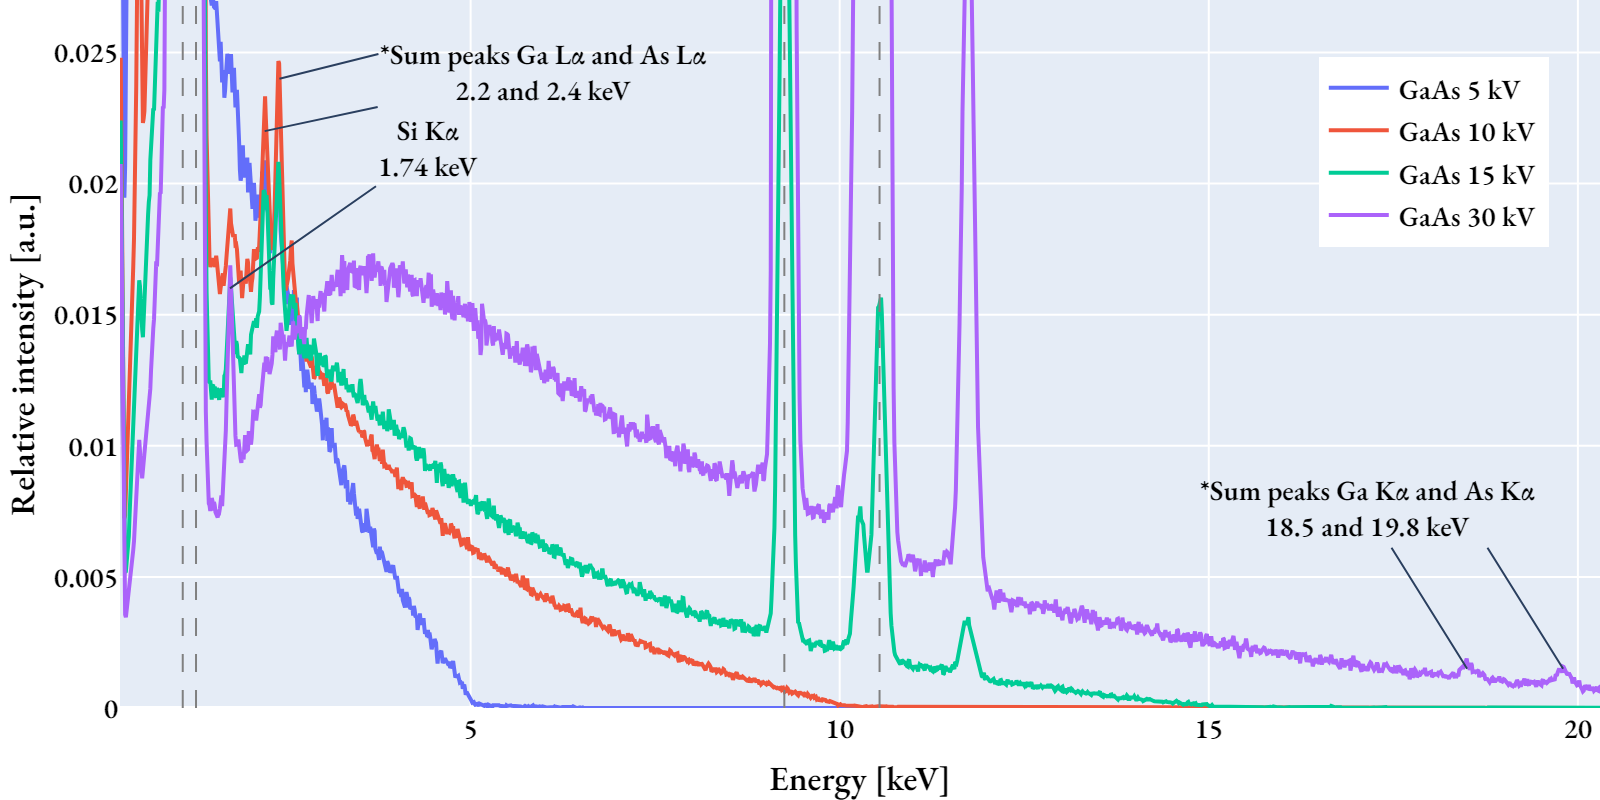
\includegraphics[width=0.90\textwidth]{figures/each_spectra/GaAs_bg_and_sum_peaks.png}
    \caption{
        A cropped in view of the GaAs bulk spectra in \cref{fig:results:Spectra_GaAs}, but with the whole x-axis to show the K-line sum peaks.
        This plot is to better visualize the background and sum peaks.
    }
    \label{fig:results:Spectra_GaAs_bg_and_sum_peaks}
\end{figure}







% The NW spectra
The GaAs nanowire spectra are shown in \cref{fig:results:Spectra_NW}.
This is the spectra with the most peaks, and contains signal from C, O, Ni, Cu, Ga, As, Si, Mo and Sb.
One of the peaks is at 0.389 keV, which could be N K$\alpha$ peak, but it could also be other elements. % Ti Ll, but no Ti K$\alpha$ peak
The Ni signal is both from the L$\alpha$ at 0.85 keV and the K$\alpha$ at 7.49 keV.
The Sb signal is from the L$\alpha$ at 3.6 keV, L$\beta$1 at 3.8 keV, and Sb L$\beta$1 at 4.1 keV. % discuss: the 3.6 peak could be smt else like ??, but the peak series show that is is Sb
The Mo signal is both from the L$\alpha$ at 2.29 keV and the K$\alpha$ at 17.47 keV, but the K peak is very weak and thus not included in the plot.
Mo is also giving a small signal at 2.02 keV, which is the Ll line.
The Cu signal is both from the L$\alpha$ at 0.92 keV and the K$\alpha$ at 8.05 keV.
The tallest peak in all four spectra is the Ga L$\alpha$ peak at 1.1 keV.
In the 5 kV spectrum the C K$\alpha$ peak at 0.26 keV is equally high as the Ga L$\alpha$ peak.
The As and Ga signals and their ratios are very similar to the GaAs spectrum signal, but the sum peaks are not visible in the NW spectra.
The Ga and As L$\alpha$ sum peaks could have been visible, but the sum peak signal coincides with the Mo L$\alpha$ peak at 2.2 keV. % discussion: the sum peaks could be missing due to lower DT.
The 10, 15 and 30 kV signal have Mo Ll peak at 2.02 keV, between Si K$\alpha$ and Mo L$\alpha$. % discussion: what is this? Sum peak? No elemet match well. or escape peak (Line - Si Ka)? Figured it was Mo Ll, but can discuss


% discussion: se most sum peaks. No escape peak, even though the Si peak from the detector is present.

% figure Spectra_NW.png
\begin{figure}[ht!]
    \centering
    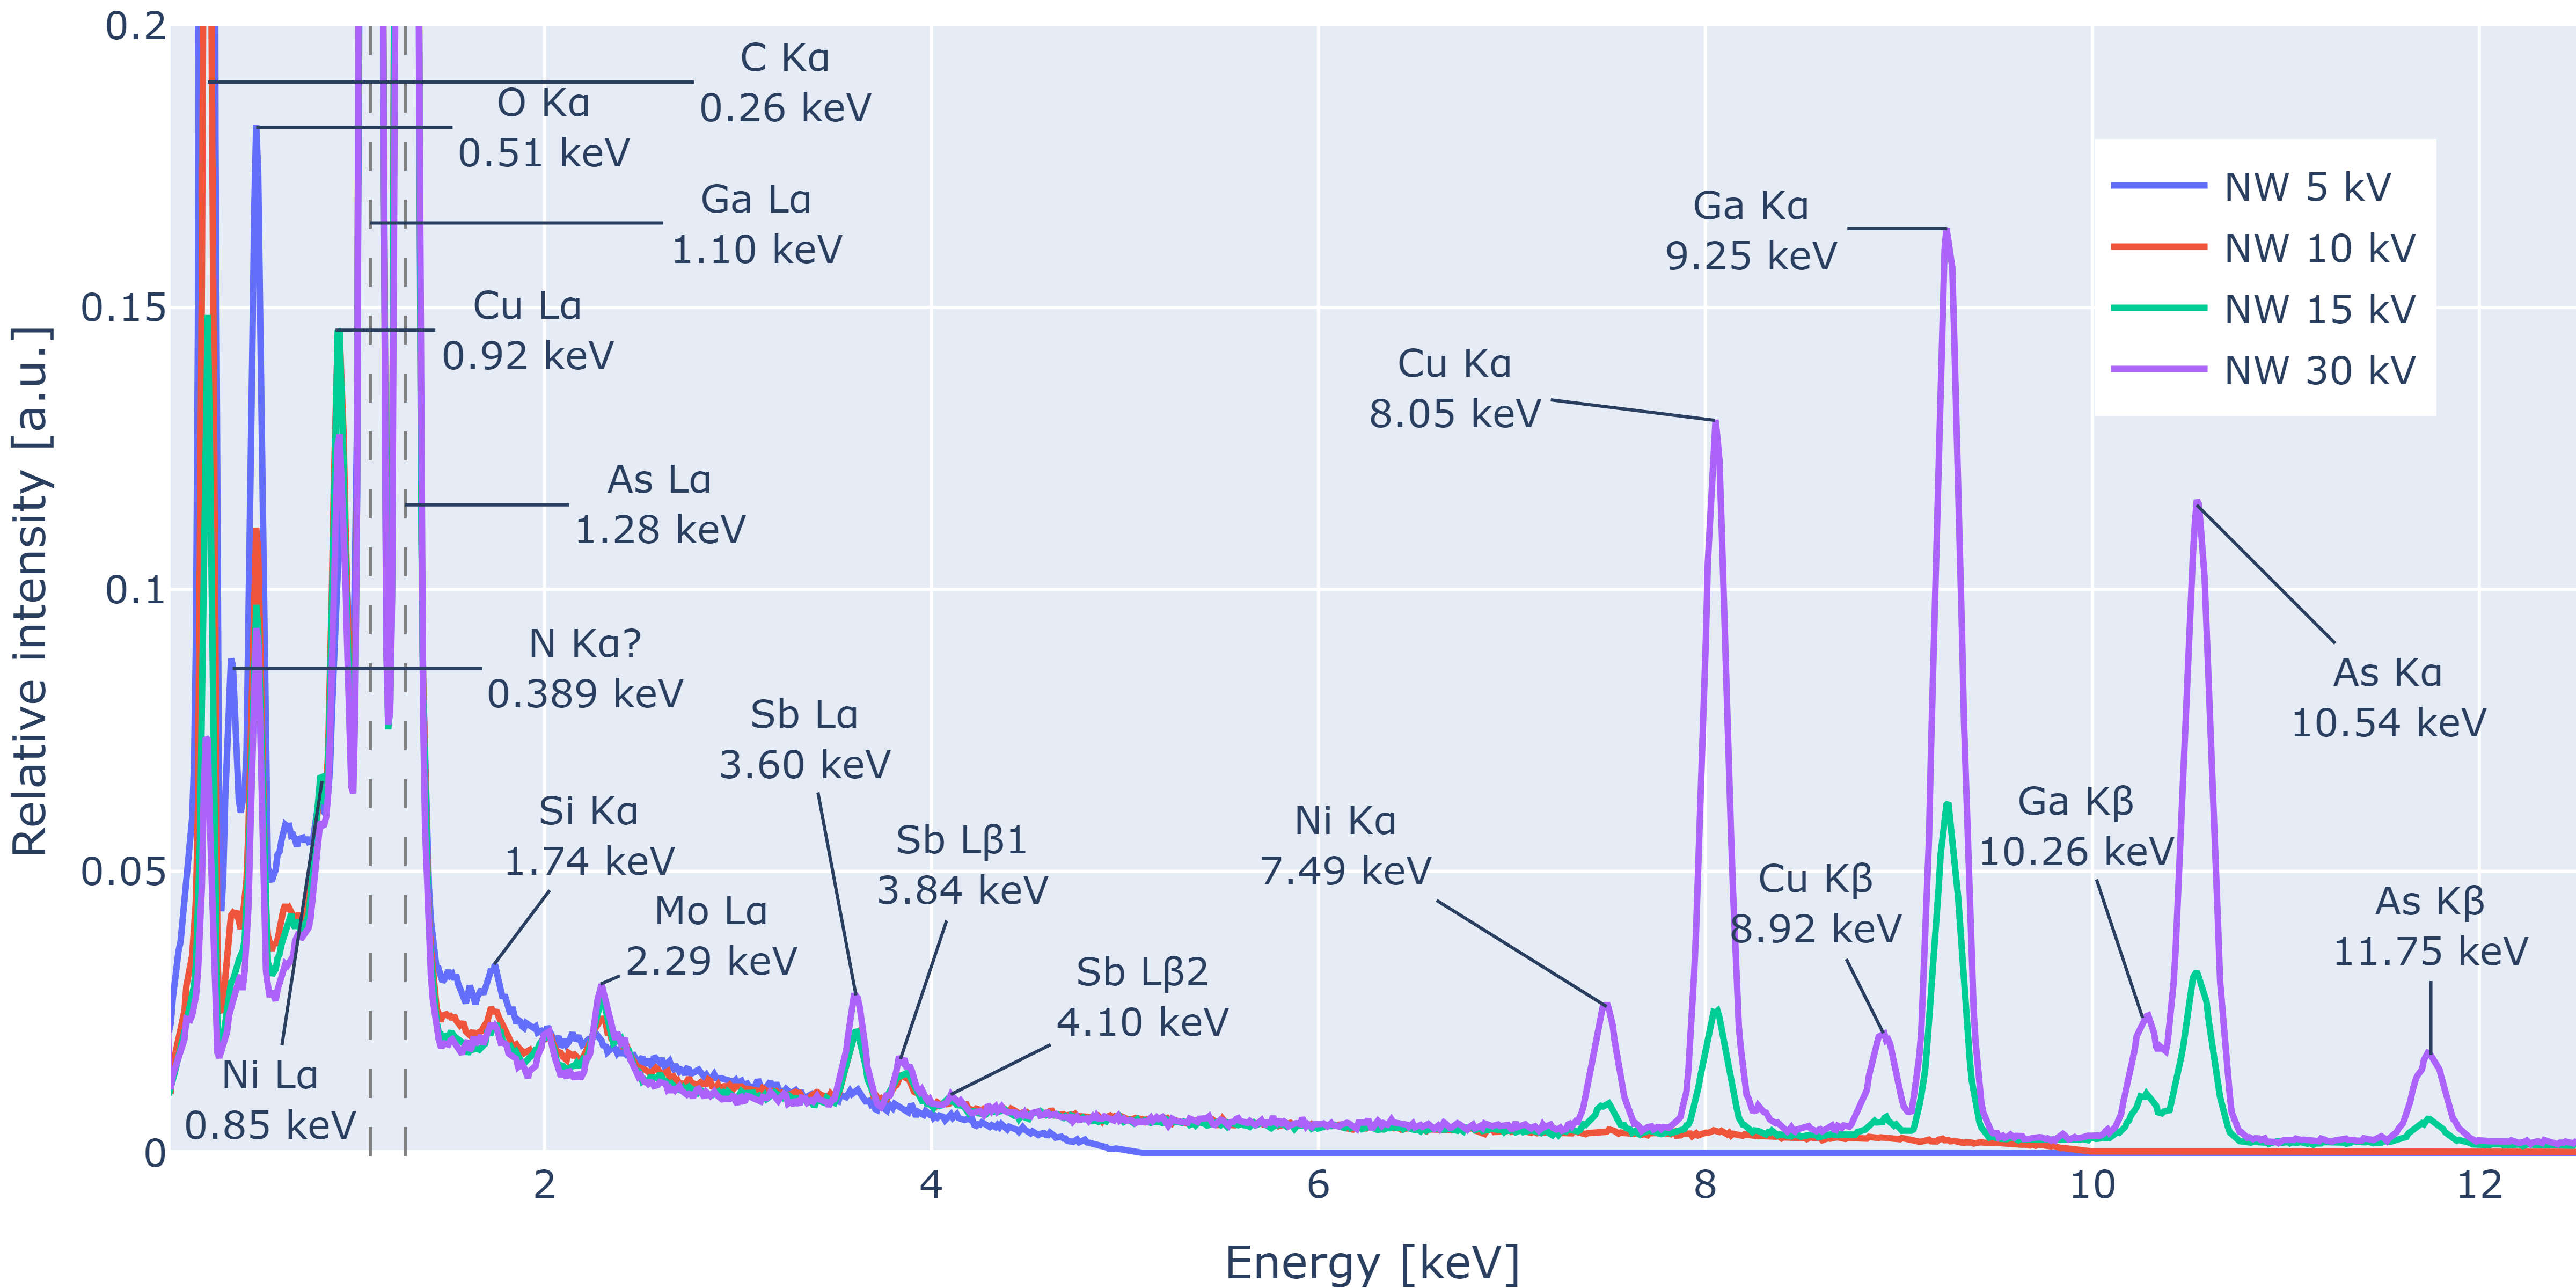
\includegraphics[width=0.90\textwidth]{figures/each_spectra/NW_everything.png}
    \caption{
        The spectra from the nanowire, taken at 5 (blue), 10 (red), 15 (green), and 30 (purple) kV.
        The peaks are annotated with the theoretical energy.
        The unknown peak is annotated with an asterisk, as it does not have a known theoretical value.
        The dashed lines mark Ga L$\alpha$ and As L$\alpha$, with relative intensities in the 30 kV spectrum at 1 and 0.82.
    }
    \label{fig:results:Spectra_NW}
\end{figure}



\newpage

\section{Quantitative results}
\label{sec:results:quantification}


The initial quantification was done on the data from the GaAs wafer in AZtec.
The results are presented in \cref{tab:initial_quantification}.
AZtec can treat the data as both TEM and SEM data, and the results were quantified with both methods.
The wafer is a 1:1 alloy of gallium and arsenic, so the atomic percent of Ga and As should be 50\% and 50\%.


% initial quantification table
\begin{table}[h]
    \centering
    \caption{
        Initial quantification of the GaAs wafer done in AZtec, treating the data as both a SEM and a TEM signal.
        The ratio in the wafer is 1:1, so the correct ratio is 50\% and 50\%, because the results are in atomic percent.
    }
    \label{tab:initial_quantification}
    \begin{tabular}{ccccc}
        $V_\textnormal{acc}$ & SEM      & SEM      & TEM      & TEM      \\
                             & Ga       & As       & Ga       & As       \\
        \hline
        5 kV                 & 46.26 \% & 53.74 \% & 54.22 \% & 45.78 \% \\
        10 kV                & 48.43 \% & 51.57 \% & 58.23 \% & 41.77 \% \\
        15 kV                & 49.32 \% & 50.68 \% & 62.13 \% & 37.87 \% \\
        30 kV                & 51.74 \% & 48.26 \% & 58.11 \% & 41.89 \%
    \end{tabular}
\end{table}

To do the quantitative analysis, HyperSpy needs k-factors from AZtec.
The k-factors for Ga and As are given in \cref{tab:results:k-factors}.
These k-factors are from the GaAs bulk wafer, and AZtec have estimated them theoretically.
% \ton{Shall I list the other k-factors for the other sample areas? I do not think I will use them, since I've only quantified the GaAs bulk wafer. But the other k-factors are results too. Eventually including NW data too, but I do not know that ratio.}
% TON answer:
% Ok to stick to GaAs.
% This is pre info and can be in methods.
% It is crucial point in quantification. The main problem and issues: need to use right k, HT dependent. Is for thin sample, prerequest, but HS let you use it anyhow.
% Conclusion could be to find a way that the user can verify k-factors or use own k-factors based on standards, like can verify calibrations.

% k-factors table
\begin{table}[h]
    \centering
    \caption{
        K-factors for Ga and As, extracted from AZtec.
        All the k-factors are theoretically estimated.
        AZtec provides either the k-factor for the L$\alpha$ or the K$\alpha$ line, and selects automatically based on the energy of the incident electrons.
    }
    \label{tab:results:k-factors}
    \begin{tabular}{ccccc}
        $V_\textnormal{acc}$ [kV] & Line      & Ga k-factor & As k-factor & $k_\textnormal{GaAs} = k_\textnormal{Ga}/k_\textnormal{As}$ \\ %Ga / As k-factor ratio \\
        \hline
        5                         & L$\alpha$ & 1.21        & 1.086       & 0.898                                                       \\
        10                        & L$\alpha$ & 1.31        & 1.223       & 0.934                                                       \\
        15                        & L$\alpha$ & 1.331       & 1.259       & 0.946                                                       \\
        30                        & K$\alpha$ & 4.191       & 3.268       & 0.780
    \end{tabular}
\end{table}


To better understand the ratios between Ga and As, the areas under the peaks in the spectra were counted.
Table \cref{tab:results:ratios} gives the ratios between the areas under the peaks for 5, 10, 15 and 30 kV.
The table compares L$\alpha$ peaks, K$\alpha$ peaks, K$\beta$ peaks and the sum of the peaks.
The table also lists the FWHM of the peaks.
The ratios are multiplied with the k-factors from AZtec to get the Cliff-Lorimer quantification results as a ratio.

\begin{table}[ht]
    \centering
    \caption{
        Ratios of Ga and As on the GaAs wafer, with the CLiff-Lorimer quantification raito.
        % The spectrum was calibrated with GaAs 30 kV.
        K$\beta$ at 15 kV was too low to be detected and is therefore not included in the table.
        The \emph{ratio} column is \emph{Ga sum} divided by \emph{As sum}.
        The \emph{CL} column is the CL quantification, done by multiplying the \emph{ratio} with $k_\textnormal{GaAs}$, from \cref{tab:results:k-factors}.
        The empty cells are for peaks where the was no k-factor or for the sum of the peaks, which have no center and no FWHM.
    }
    \label{tab:results:ratios}
    \begin{tabular}{ccccccccc}

        Peak                         & CL    & Ratio & Ga center & As center & Ga FWHM & As FWHM & Ga sum  & As sum \\
                                     &       &       & [keV]     & [keV]     & [eV]    & [eV]    &         &        \\
        \hline
                                     &       &       &           &           &         &         &         &        \\

        5 kV                         &       &       &           &           &         &         &         &        \\
        L$\alpha$                    & 1.151 & 1.282 & 1.101     & 1.288     & 74.010  & 80.921  & 75.462  & 58.844 \\
        \hline
                                     &       &       &           &           &         &         &         &        \\
        10 kV                        &       &       &           &           &         &         &         &        \\
        L$\alpha$                    & 1.349 & 1.444 & 1.100     & 1.287     & 73.841  & 80.827  & 76.222  & 52.770 \\

        \hline
                                     &       &       &           &           &         &         &         &        \\
        15 kV                        &       &       &           &           &         &         &         &        \\
        L$\alpha$                    & 1.579 & 1.669 & 1.100     & 1.287     & 73.830  & 81.137  & 77.001  & 46.146 \\
        K$\alpha$                    &       & 2.445 & 9.253     & 10.536    & 155.080 & 181.951 & 6.013   & 2.459  \\
        % K$\beta$       & 1.000 & 10.536         & 10.536         & 181.951      & 181.951      & 2.459   & 2.459  \\
        L$\alpha$+K$\alpha$          &       & 1.708 &           &           &         &         & 83.014  & 48.605 \\
        % L$\alpha$+K$\alpha$+K$\beta$ & 1.674 &            &            &          &          & 85.473  & 51.065 \\

        \hline
                                     &       &       &           &           &         &         &         &        \\
        30 kV                        &       &       &           &           &         &         &         &        \\
        L$\alpha$                    &       & 2.279 & 1.098     & 1.287     & 72.309  & 80.849  & 76.465  & 33.546 \\
        K$\alpha$                    & 1.301 & 1.678 & 9.253     & 10.542    & 157.799 & 168.238 & 58.718  & 34.994 \\
        K$\beta$                     &       & 1.603 & 10.276    & 11.736    & 171.804 & 185.034 & 8.821   & 5.503  \\
        L$\alpha$+K$\alpha$          &       & 1.972 &           &           &         &         & 135.184 & 68.540 \\
        L$\alpha$+K$\alpha$+K$\beta$ &       & 1.945 &           &           &         &         & 144.004 & 74.042
    \end{tabular}
\end{table}


One of the adjustments explored was the affect of the calibration on the quantification.
Using different the calibrations in \cref{tab:results:calibrations} gave different quantification results when using CL in HyperSpy. % discussion: Issue with using Clif-Lorimer since I have bulk and not thin sample. But the own produced CL just misses harder, it does not break down completely.
The results are presented in \cref{tab:results:calibration-quantification}.
The same method was used on all spectra, but the quantification on 10 and 15 kV are obviously wrong.





% table with peak accuracy

\begin{table}[ht]
    \centering
    \caption{
        Quantification with different calibration methods.
        The quantification is done by in HyperSpy with Cliff-Lorimer method.
        The CL method is for this samples, while the GaAs wafer used here is a bulk sample.
        AZ is the AZtec calibration.
        HS is the HyperSpy calibration.
        GaAs is the calibration on the GaAs 30 kV spectrum.
        The accuracy of the quantification is the deviation from 50\%, because the sampled area is 1:1 GaAs wafer.
    }
    \label{tab:results:calibration-quantification}
    \begin{tabular}{cccccc}
        Vacc & Element & Line & AZ     & HS     & GaAs   \\
        \hline
        5    & As      & L    & 44.81  & 44.29  & 44.19  \\
        5    & Ga      & L    & 55.19  & 55.71  & 55.81  \\
        10   & As      & L    & 100.00 & 100.00 & 100.00 \\
        10   & Ga      & L    & 0.00   & 0.00   & 0.00   \\
        15   & As      & L    & 5.23   & 4.39   & 5.87   \\
        15   & Ga      & L    & 94.77  & 95.61  & 94.13  \\
        30   & As      & K    & 56.25  & 57.14  & 59.02  \\
        30   & Ga      & K    & 43.75  & 42.86  & 40.98
    \end{tabular}
\end{table}

% affect of calibration
% accuracy on quantification


% affect of peak and background modelling
% both errors and the quantification accuracy
% could model as other than Gaussian? Discussion




% Conclusion: update dispersion and offset for the APREO?